\documentclass[12pt]{article}
\usepackage{multirow,sectsty}
\usepackage[margin=1in]{geometry}
\usepackage{setspace}
\usepackage{subfigure,graphicx}
\usepackage{amsmath,amsthm,amsfonts, amssymb}
\theoremstyle{definition} \newtheorem{definition}{Definition} 
\usepackage{linguex}
\usepackage[english,greek]{betababel}
\usepackage{tikz}
\usetikzlibrary{arrows,automata,chains,matrix,positioning,scopes}

%\usepackage{mathspec}
%  \setmainfont{Gentium Plus}
%\usepackage{fontspec}
%\setmainfont{Arial}

\usepackage[only, llbracket,rrbracket]{stmaryrd}
\newcommand{\sem}[1]{\ensuremath{\{ #1 \} }}
\newcommand{\pair}[1]{\ensuremath{\langle #1 \rangle}}
\newcommand{\la}{\ensuremath{\lambda}}
\newcommand{\inter}[1]{\ensuremath{\llbracket#1\rrbracket}}

\usepackage{natbib}
\bibliographystyle{mcbride}


%%%%%%%%%%%%%%%%%%%%%%%%%%%%%%%%%%%%%%%%%%%%
\begin{document}

\title{Cycles and Stability in Linguistic Signaling}
\author{Christopher Ahern \vspace{5mm} \\ 
Dissertation proposal\\ Submitted May 5, 2014\\
Department of Linguistics, University of Pennsylvania \vspace{5mm} \\
Dissertation Supervisor: Robin Clark\\
Proposal Committee: Anthony Kroch (chair), Mark Liberman, Florian Schwarz}
\date{}

\maketitle

% \begin{center}
%  A Dissertation Proposal\\
%  Submitted April 9, 2014\\
% Department of Linguistics, University of Pennsylvania\\
% \end{center}


\section{Introduction}

Language change is evidenced by a difference between the linguistic expressions of one generation and the next. Given that the output from one generation serves as the input to the next, both language acquisition and use are crucial to the process of change. While the input to acquisition arises from the interplay of many factors, it is not arbitrary. Rather, it is governed by a \emph{pragmatic andnce} that ``underlies the ability to use [\emph{grammatical competence}] along with the conceptual system to achieve certain ends or purposes'' \citep[59]{chomsky1980rules}. In the terms of \cite{chomsky1986knowledge}, the process of language acquisition maps the \emph{E-Language} of one generation to the \emph{I-Language} of the next, whereas pragmatic competence is what governs the mapping from each generation's \emph{I-Language} to its \emph{E-Language}.

In the Gricean tradition \citep{Grice:1975, Levinson:1983, Horn:1984}, this pragmatic competence has been framed in terms of speakers' beliefs, preferences, and intentions. Linguistic expressions are used according to a \emph{Cooperative Principle} whereby interlocutors are taken to make the appropriate contribution to the conversation at the appropriate time towards ``the accepted purpose or direction of the talk exchange'' \citep[26]{Grice:1975}. This framework deftly captures the systematic relationship between what is \emph{said} and what is \emph{meant}, but is clearly an idealization: speakers and hearers might, but need not have the same preferences or goals in a given exchange.   This dissertation aims at understanding the consequences of loosening the assumption of Gricean commonality. It will examine how differences in speakers' and hearers' preferences might impact the use and acquisition of linguistic signals over time. 

At the center of this endeavor will be a diachronic process that implicates both use and acquisition, the development in the expression of negation over time known as \emph{Jespersen's Cycle} \citeyearpar{jespersen:1917}. The main components of this dissertation address the main components of the cycle in turn. First, we consider how the expression of negation transitions from a purely preverbal negator with an optional \emph{emphatic} postverbal element towards a system with obligatory preverbal and postverbal elements. We present a formal model that derives this transition from even a slight preference for exaggeration on the part of speakers. If speakers prefer hearers' response to the emphatic form, then the optional postverbal element will increase in use. On the way up it experiences a kind of \emph{rhetorical devaluation} \citep{dahl:2001}, and is at least partially \emph{bleached} of its emphatic force because, simply put, to ``to emphasize everything is to emphasize nothing'' \citep{kiparsky-
condoravdi:2006}. Second, we consider how the expression of negation can shift from the original preverbal negator to the new, increasingly-used, postverbal element. We outline the conditions under which a learner would posit that the postverbal element is a negator in its own right. If the preverbal element appears in contexts where it does not itself express negation, this provides evidence that postverbal element expresses negation and for the eventual loss of the preverbal element entirely. We consider the interaction between these two components of the cycle.

The main contributions of this line of research are the following. First,  it extends recent work in game-theoretic pragmatics that has begun to explore the broader space of possibly divergent preferences \citep{benz-jager-van-rooij:2006, franke:2008, franke-etal:2012, de-jaegher-van-rooij:2013}. This can be taken as a straightforward generalization of the Gricean program to understand the use of linguistic expressions not just as something ``all or most do \emph{in fact} follow but as something that it is \emph{reasonable} for us to follow, that we \emph{should not} abandon'' \citep[29]{Grice:1975}.  Second, it incorporates this perspective into the use of linguistic signals over time. In particular, it suggests how Grice's criterion of reasonability might cut both ways: there are some patterns of use that we \emph{should} and \emph{do} abandon. Differentiating the cases where we expect stability from those where we expect change adds to a broader causal theory of language change \citep{yang2000internal}. 
Namely, it offers an additional \emph{internal} force of language change, which derives from a shared pragmatic competence. In the case of Jespersen's Cycle it suggests how morphosyntactic change might arise through a kind of communicative bleaching.   More broadly, it offers insight into the interaction between use and acquisition implicit in the common representation of iterated language change as in Figure \ref{trans}.

\begin{figure}
\begin{center}
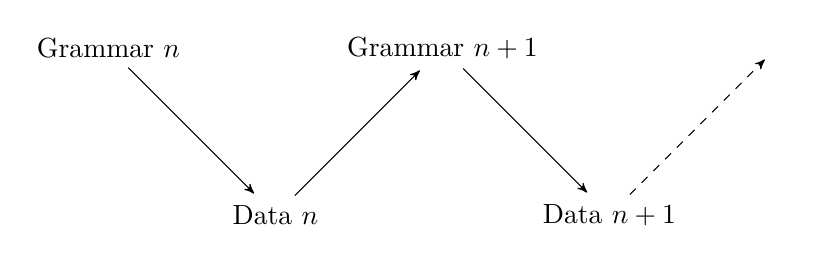
\begin{tikzpicture}[->,>=stealth',shorten >=1pt,auto,node distance=3cm]
  \node (A)      {Grammar $n$};
  \node (B) [below right of=A]  {Data $n$};
  \node (C) [above right of=B] {Grammar $n+1$};
  \node (D) [below right of=C] {Data $n+1$};
  \node (E) [above right of=D] {};
\path[->] (A)  edge node {} (B)
  (B) edge node {} (C)
  (C) edge node {} (D)
  (D) edge[dashed] node {} (E);
\end{tikzpicture}
\end{center}
\caption{The iterated process of language change through acquisition and use}
\label{trans}
\end{figure}

The rest of the proposal is structured as follows. Section \ref{Background} offers an overview of Jespersen's Cycle.  We consider the two major approaches to the change, as a \emph{pull-chain} or a \emph{push-chain}. We adopt the latter given that the driving force behind the cycle appears to be pragmatic in nature, stemming from continuous loss and renewal of emphatic negation. We then consider a natural simplification of Eckardt's \citeyear{eckardt2006} analysis of emphatic negation. In Section \ref{Signaling} we develop the mathematical framework that will be used to explicitly connect the analysis of emphatic negation with the cycle. In Section \ref{Cycles} we apply the framework and consider the cycle as a signaling game played in a population where the interests of speakers and hearers slightly diverge. We determine the conditions for the existence of different kinds of equilibria, and the impact of the introduction of new signals under the game dynamics. Finally, in Section \ref{Stability} we 
determine how the change brought about by use might impact acquisition over time. We suggest different mechanisms that might impact the amount of evidence available to learners at various points in time and how this shapes the trajectory of the change.

\section{Background}
\label{Background}

\subsection{Jespersen's Cycle}

Originally coined by \cite{dahl:1979}, \emph{Jespersen's Cycle} refers to an observation of the expression of negation over time for several European languages. While more recent work has established its cross-linguistic prevalence \citep{vanGelderen2008negative}, the most widely-cited form of the  cycle can be drawn from Jespersen's original observations of, among others, English and French. 

The first stage is that of purely preverbal negation. This is seen in Old English and Old French, where ``ne'' expresses negation alone.

\exg. Ic ne secge\\
      I neg say\\
      (Old English)

\exg. Jeo ne dis\\
      I neg say\\
      (Old French)

This is followed by a stage of embracing or bipartite negation where a postverbal negative reinforcer is added. This is seen in Middle English and Middle French, where ``ne'' is reinforced by ``not'' and ``pas'' in the two languages.


\exg. I ne seye not\\
      I neg say neg\\
      (Middle English)

\exg. Je ne dis pas\\
      I neg say neg\\
      (Middle French)

Finally, there is the stage of purely postverbal negation. This is seen in Early Modern English and Present-day Colloquial French, where ``ne'' is lost.

\exg. I say not\\
      I say neg\\
      (Early Modern English)

\exg. Je dis pas\\
      I say neg\\
      (Present-day Colloquial French)


A more articulated model captures the intuition that there are transitions between these stages \citep{vanderAuwera2009}. That is, between the purely preverbal and embracing negation there is a period of optional embracing negation; between the obligatory embracing negation and purely post-verbal negation there is a period of optional embracing negation. Where parentheses are taken to indicate optionality, the stages can be represented schematically as the following.

\begin{center}
\begin{enumerate}
     \item \textsc{n V}
    \item \textsc{n V (n)}
    \item \textsc{n V n}
    \item \textsc{(n) V n}
    \item \textsc{ V n}
\end{enumerate}
\end{center}
Note that this does not preclude the coexistence of all three forms synchronically. For example, we do indeed find instances of all three forms in variation: \textsc{n V} $\sim$ \textsc{n V n} $\sim$ \textsc{V n} \citep{schwenter2005, schwenter2006}. We might then, at least for the moment, consider this a general trajectory over time.

In Present-day English there seems to have been a partial re-establishment of the initial state due to the loss of V-to-T raising, the emergence of \emph{do}-support, and the contraction of negation.

\exg. I don't say\\
      I do-neg say\\
      (Present-day English)

Thus, the cyclic nature of the cycle can be attributed to an eventual return to original syntactic state. However, in Present-day Colloquial French there has yet to be such a change towards the original syntactic state of purely preverbal negation. Nor is any such return guaranteed to occur. It seems strange to call something a cycle if it never returns to the point of origin. A resolution to this conceptual problem lies in considering the potential causes of the cycle. The two approaches in the literature regarding the cause of the change can be summarized as \emph{push-chains} and \emph{pull-chains}.

\subsubsection{Pull-Chain}
In Jespersen's own words, the transition between the stages is a matter of \emph{weakening} and \emph{strengthening}.

\begin{quotation}
The history of negative expressions in various languages makes us witness the following curious fluctuation: the original negative adverb is first weakened, then found insufficient and therefore strengthened, generally through some additional word, and this in its turn may be felt as the negative proper and may then in course of time be subject to the same developments as the original word. \citep[4]{jespersen:1917} 
\end{quotation}
In the case of a pull-chain analysis, the preverbal negation has a tendency to not receive main stress and thus becomes a clitic. Given the importance of the distinction between affirmation and negation, some additional word is used ``to increase the phonetic bulk'' of the negative signal to bolster its perception \citep[14]{jespersen:1917}. That is, some new marker is \emph{pulled} into expressing negation because of the weakening of the original preverbal negator.

The prevalence of phonetic weakening suggests we should be skeptical of its role in any particular morphosyntactic change. There is ample evidence of phonetic weakening not leading to morphosyntactic change, and morphosyntactic change in the absence of any precursory phonetic weakening. More pertinent to the case at hand, \cite{posner1985} argues from Italian dialect data that apparently weak preverbal negators are not necessarily supplemented by some additional element. If phonetic weakening is not sufficient for the cycle, then this suggest that a pull-chain scenario is unlikely.

\subsubsection{Push-Chain}

Perhaps unsurprisingly, Jespersen prefigured the other major conception of the cycle insofar as he took weakening and strengthening to be both phonetic and semantic in nature.  In the latter case, which Jespersen thought to be the more frequent, some additional word is used ``to make the negative more impressive as being more vivid or picturesque'' \citep[15]{jespersen:1917}. This intuition is exactly what more recent theories have referred to as emphasis (\citealt{detges-waltereit2002, hopper-traugottt2003, eckardt2006, kiparsky-condoravdi:2006}, \emph{inter alia}).  More precisely, the incoming form of embracing negation is emphatic in comparison to the original form of preverbal negation. 

On this second account, the increasing use of the postverbal emphatic element eventually leads to its loss of emphatic force. As \cite{kiparsky-condoravdi:2006} so eloquently note, ``to emphasize everything is to emphasize nothing.'' The directionality of the change then proceeds from the introduction of the post verbal element and its transition towards being obligatory. The new element potentially takes over the expression of negation in its own right, \emph{pushing} the original negator out. While this approach to the cycle often takes the loss of the preverbal negator as a given, it should be noted that this is most definitely not guaranteed. That is, while the postverbal element may increase in frequency and lose its emphasis, it need not necessarily come to be the sole expression of negation and push the preverbal element out. As a case in point, \cite{kiparsky-condoravdi:2006} present evidence from the history of Greek for the stability of a single preverbal negator over multiple centuries alongside 
several postverbal elements that first convey emphatic and then plain negation. This provides further evidence that a pull-chain scenario is untenable given that phonetic weakening is neither necessary nor sufficient for the cycle.

The push-chain scenario, however, offers a new perspective on the pull-chain mechanism. That is, it suggests the phonetic reduction of the preverbal element not as the cause of the change, but rather as an effect of it. The phonetic bulk of the preverbal negator may be crucial in determining if and when the expression of negation is identified elsewhere. For example, a less substantial element might not be perceived, yielding evidence that it does not express negation, whereas a more substantial element might provide  sufficient evidence for its status as the expression of negation. It is unsurprising that the relevant preverbal negator in Greek constitutes a heavy syllable, which would arguably have enough phonetic heft to be identified.

Additionally, the push-chain suggests a particular interpretation of what is being pushed. That is, the form of plain negation is being pushed out by the form of emphatic negation. The cycle can be thought of as  essentially semantico-pragmatic in nature. It stems from the loss and renewal of emphatic negation due to pragmatic pressures.  This is obviously not to say that the relevant morphosyntactic repercussions are unexpected; the surprising cross-linguistic regularity of occurrence is what prompted Jespersen's original observation. Rather, it suggests that the use of negation under pragmatic pressures can, and often does have morphosyntactic consequences. In what follows we will consider the implications of this characterization of the cycle. We start with a characterization of emphatic negation.


\subsection{Emphatic Negation}

Elements recruited to induce emphasis are by and large \emph{negative polarity items}, overwhelmingly drawn from the set of \emph{minimizers} (e.g. ``not a drop'', ``not a hair'') and \emph{generalizers} (e.g. ``not ever'', ``not at all'') \citep{horn:1989}. These can be seen in the examples of the cycle in English and French above. In the case of English, ``not'' comes from Old English ``nawiht'' (\emph{literally} ``no'' + ``thing, creature, being''). In the case of French, ``pas'' comes from ``step'', and in fact still has this separate meaning in non-negative contexts. Other sources include, but are not limited to indefinite pronouns (e.g. ``no one'') and negative adverbs (e.g. ``never'') (cf. \citealt{horn:1989,vanGelderen2008negative}).

\cite{eckardt2006} draws on a variant of the analysis presented in \cite{krifka1995polarity} to give a particularly appealing account of how these NPIs are used to express emphatic negation. The basic intuition is that emphatic negation arises through the occurrence of NPIs under emphatic focus.  Theories of \emph{focus} draw on the notion of alternatives, incorporating what could have been said into the computation of focus sensitive construction \citep{rooth1992}. NPIs pick out extremal elements of the relevant set of alternatives, and emphasis indicates that this choice is in some sense surprising. This account recommends itself not only because it integrates the relevant material into the compositional machinery of the semantics, but it does so through independently motivated mechanisms. We present the two components of this account in turn, following Eckardt's exposition unless otherwise noted. We then offer a slightly simpler means of deriving the impact of emphatic negation.

The first component of Eckardt's account draws on the notion of alternatives induced by focus. In addition to the ordinary semantic interpretation, an expression $E$ also has a focus driven semantic interpretation. We can represent the first by \inter{E}$^o$ and the second by \inter{E}$^f$. The ordinary interpretation of an expression is as would be expected given the usual semantic machinery. In contrast, the focus  driven interpretation is sensitive to the presence of an abstract focus feature $f$. The focus driven interpretation of the abstract focus feature yields a set consisting of the ordinary semantic value of the expression and the set of salient alternatives in the context: $\{F_1, F_2, F_3...\}$.  Thus, the presence or absence of a focus feature gives rise to the following possibilities.

\ex. \inter{E}$^f$ $= \{\inter{E}^o\} $

\ex. \inter{E_f}$^f$ $= \{\inter{E}^o, F_1, F_2, F_3...\} $

The set of alternatives is restricted to be of the same logical type as the expression. So, for example, nouns evoke alternative entities, transitive verbs evoke binary relations between entities, and so forth. In essence, this simply captures the intuition that the realization of focus generates a set of alternatives when it occurs, but has no effect when it does not. Similarly, the abstract focus feature is, so to speak, invisible to the ordinary semantic interpretation.

Computing the meaning of a complex expression $AB$, which contains a focus marked element, is accomplished by the following  rule of evaluation, where $\infty$ indicates a suitable method of semantic composition, 

\ex. \inter{AB}$^f = \{ A_i \infty B_j | A_i \in \inter{A}^f, B_j \in \inter{B}^f \} $

When no subexpression is focus marked, this simply results in ordinary semantic composition. That is, the focus driven interpretation simply yields the normal functional application, or predicate modification, of the two subexpressions. When a subexpression is focus marked this generates a set of alternatives, which then all undergo the appropriate semantic composition.

As a simple example, consider the following sentence where $f$ indicates the abstract focus feature, which is reflected in English prosody via prominent stress.

\ex. John$_f$ knows the number.

The components of the sentence are then the following, supposing that the individuals in the context are John, Joe, and Jim.

\ex. \inter{John_f}$^f = \{ \inter{John}^o, Joe, Jim \} = \{ John, Joe, Jim \}$

\ex. \inter{\text{knows the number}}$^f = \{ \inter{\la x . know(x, \text{the number})}^o \} = \{ \la x . know(x, \text{the number}) \}$

The composition that results yields the set of alternatives of all individuals that could know the number.

\ex. \inter{\text{knows the number}}$^f$(\inter{John_f}$^f) = \{$ John knows the number, Joe knows the number, Jim knows the number $\}$


The second component of Eckardt's account is the notion of emphatic assertion. In this case, the resulting effect of emphatic assertion is taken to be akin to a tacit ``even''.  For example, consider the following sentence.

\ex. Even John$_f$ knows the number.

In addition to the assertion that John indeed knows the number, it implicates that all of the alternatives are also true, and, most importantly, that the asserted proposition is the most surprising or striking of all the alternatives.

It is this last aspect which is taken to be crucial in emphatic assertions. The effect of emphasis can be encoded as an operator, the application of which yields both the asserted content, the ordinary semantic interpretation of the sentence, along with an implicature regarding the relation between the asserted content and all its alternatives. Where $P$ is taken as some measure of expectation in a given context, the effect can be represented as the following.\footnote{This is a trivial reformulation of \cite{eckardt2006}, which is a slight departure from that of \cite{krifka1995polarity}. The latter requires that the asserted statement be more surprising than the conjunction of all other alternatives. Nothing hinges on this difference, but here we adopt the less stringent criterion.}

\ex. \textbf{emph}(S) \\ asserts: \inter{S}$^o$ \\ implicates: $\forall S' \in \inter{S}^f . P(\inter{S}^o) \leq P(\inter{S'}^o)$

That is, an emphatically asserted utterance carries with it the implicature that it is somehow surprising or unexpected in comparison to its alternatives.

With both components, we can evaluate a sentence with an NPI.

\ex. Anna did not drink [a single drop]$_f$

This sentences gives rise to the set of alternative propositions.

\ex. \inter{S}$^f$ = $\{$ `Anna did not drink a single drop', `Anna did not drink a glassful', `Anna did not drink a barrelful', `Anna did not drink a swimming pool-ful'...$\}$

Emphatically asserting this sentence leads to the implication that, of these alternatives, the proposition that is actually asserted is the most striking or unexpected.

\ex. \textbf{emph}(Anna did not drink [a single drop]$_f$) \\ asserts: Anna did not drink a single drop. \\ implicates: This is surprising or unexpected relative to what she could have drunk.

NPIs generate alternatives through focus, and emphatic focus leads to the implication that the asserted proposition is surprising or unexpected in comparison to its alternatives. Taken together, these components allow for the effects of emphatic negation to be derived pragmatically.

While these components together yield the desired effect of emphatic negation, a perhaps more parsimonious account lies in the nature of the alternatives generated by NPIs. That is, unlike the alternatives induced by focus marking of an individual, NPIs introduce alternatives that are ordered along a scale according to semantic entailment.

Scales underpin our reasoning about the relationship between ordered sets of propositions. For example, imagine a set of puzzles ordered by degree of increasing difficulty: $y_1 < y_2 < ... < y_n$. Positive and negative claims regarding an individual's ability to solve a particular puzzle allow for inferences regarding that same individual's ability to solve other puzzles. For example, consider the following.

\ex. John can solve puzzle $y_i$.

\ex. John can't solve puzzle $y_i$.

From the first, we can infer that John can solve all easier puzzles; he can solve $y_j$ for all $j \leq i$. From the second, we can infer that John cannot solve any harder puzzles; he cannot solve $y_j$ for any $j \geq i$. The latter contexts are \emph{scale-reversing} allowing inferences from low values on the scale to high values, whereas the former are \emph{scale-preserving} allowing inferences from high values on the scale to low values \citep{fauconnier1975}.

NPIs pick out the low end of a particular scale and allow us to reason about propositions higher in the scale. In contrast with ordinary negation, emphatic negation signals two things \citep{kadmon-landman1993any}. First, there is a reduced tolerance to exceptions. For example, in the case of a cook making dinner for a large group of people, the amount of potatoes that would be relevant is quite large. We can imagine the following exchange.

  \ex. \a. Will there be French fries tonight?
       \b. No, I don't have potatoes.
       \b. Maybe you have just a couple of potatoes that I could fry in my room.
       \b. Sorry, I don't have \textsc{any} potatoes.

Emphasis \emph{widens} the interpretation of potatoes from quantities relevant to a large group to quantities relevant to even a single person.
 
Second, emphasis yields a stronger statement. For example, in the case of the following threats, the latter is clearly the stronger prohibition.

  \ex. \a. If you move, I'll shoot.
       \b. If you budge an inch, I'll shoot.

It is clear that either form of the threat allows for a certain amount of pragmatic slack in interpretation: being shot for blinking would seem rather ungenerous. However, there is still a clear relationship between the two. While scratching an itch might not be advisable in either situation, it as at least less inadvisable under the former than the latter. In all those situations where the first threat would be carried out we would expect the second to be as well, but not vice versa. In this sense, emphasis \emph{strengthens} the interpretation of a given statement.

The basic intuition that connects the two effects of NPIs is that they signal something about how strictly the meaning is to be interpreted (cf. \citealt{lewis1970,landman1991}). In the examples above, this determines what it means to have potatoes or what counts as moving. We will refer to this contextually determined value as the \emph{standard of precision}. Such standards of precision stand in a particular relation to each other \citep{krifka1995polarity}. Namely, for two standards of precision, $t_i$ and $t_j$, we might say that one is stricter than the other, $t_i \prec t_j$ just in case the extensions of a given property, $\alpha$, is preserved under a loosening of the standard. 

\ex. $t_i \prec t_j$ if and only if $\alpha_j \subset \alpha_i$

This simply means that anything that holds at a stricter standard holds at a looser standard, but not necessarily vice versa. So, not having potatoes for a single person means that you still do not have enough potatoes for fifty people. But, not having potatoes for fifty people does not mean that you do not have enough for just one person. Likewise, scratching an itch might not get you shot at the looser standard, but it certainly could at the stricter one.

Intuitively, an NPI makes negation emphatic because it signals a stricter standard than might be normally expected. It suggests that the speaker has evidence for making the assertion even under some stricter standard of interpretation. While plain negation might be compatible with a wide range of standards, emphatic negation picks out a much narrower range standards. Namely, it picks out an extremely high standard, if not the highest. In this sense, emphatic negation is surprising because it is particularly informative relative to plain negation \citep{israel1998,israel2001}. This is, of course, not an immutable fact about emphatic negation. It is exactly the loss of informativity that is at the center of Jespersen's Cycle. The question is then why emphatic negation, and the information it conveys, are subject to this continual erosion. In the next section we will lay out a formal framework for exploring this question.


\section{Signaling}
\label{Signaling}

Here we outline the mathematical framework that will be used subsequently. First, signaling games are introduced. The relevant structures and definitions are presented along with a simple example. Second, we consider a particular solution concept for the behavior of a population and relate it to the previously given example. This allows us to determine the existence and characteristics of equilibria. Finally, we specify a game dynamics which determines how a population of agents changes over time. We note its relation to the solution concept, and where it adds to the model.

It should be noted that there are multiple traditions that have contributed to the development of signaling games. In the Economic tradition the work of \cite{harsanyi:1967,harsanyi:1968a,harsanyi:1968b} on games of incomplete information and Spence's \citeyearpar{spence:1973} model of job signaling have been central. In the Philosophical tradition, the work of \cite{lewis:1969} has been the most influential. His response to the Quinean skepticism that meaning could arise by convention has had the most direct impact on Linguistics. This account, however, rests on the assumption that speakers and hearers have perfectly-aligned interests.  This assumption will figure in the exposition of this section, mostly for the simplicity it affords us in the examples. In the next section we turn towards the consequences of loosening it.


\subsection{Signaling Games}

Signaling games offer an intuitive model of communication between agents.  A signaling game consists of two players, a sender and a receiver. The sender has some private piece of information, $t \in T$, drawn according to some commonly known probability distribution, $\delta$. The piece  of information can be thought of as some fact about the state of the world. For example, we might think of it as information that the sender wants to convey to the receiver. The sender chooses a message, $m \in M$, to send to the receiver.   The receiver does not know what state of the world actually holds and must choose an action, $a \in A$, as an interpretation of the message sent. That is, the receiver is faced with the problem of inferring the state of the sender given the message.

The outcome of the game is determined by the state of the sender, the message sent, and the action taken by the receiver. The sender and the receiver have preferences over these outcomes, which are given by utility functions, $U_S$ and $U_R$ respectively, which map outcomes to real numbers:\footnote{It should be noted that utilities are only important insofar as they represent an ordinal ranking over outcomes, and should only be interpreted as such. In other words, there is nothing particularly special about $0$ and $1$ as opposed to say $3.277$ and $110$ other than the fact that in both cases the first is less than the second. Generally speaking, where possible, it is best to keep things algebraic to avoid imputing anything more meaningful.} $U_S,U_R:T \times M \times A \rightarrow \mathbb{R}$.

As a simple example of a signaling game, consider the case where there are two states, two messages, and two actions: $T = \{t_1, t_2 \}$, $M = \{m_1, m_2 \}$, and $A = \{a_1, a_2 \}$. We can represent the structure of the game in \emph{extensive form} as in Figure \ref{SG1}. The uppermost node, labeled $\delta$, determines the likelihood of either of the two states occurring. The lines from the uppermost node represent one state or the other obtaining. The nodes labeled $S$ indicate the points in the game where the sender makes a decision regarding which message to send. The nodes labeled $R$ indicate the points where the receiver must make a decision regarding how to interpret the message. The dashed lines between receiver nodes indicates that the receiver is uncertain as to which state holds after hearing a given message. The nodes at the bottom represent the outcome and the players' preferences, as determined by the utility functions.

\begin{figure}[!ht]
\centering
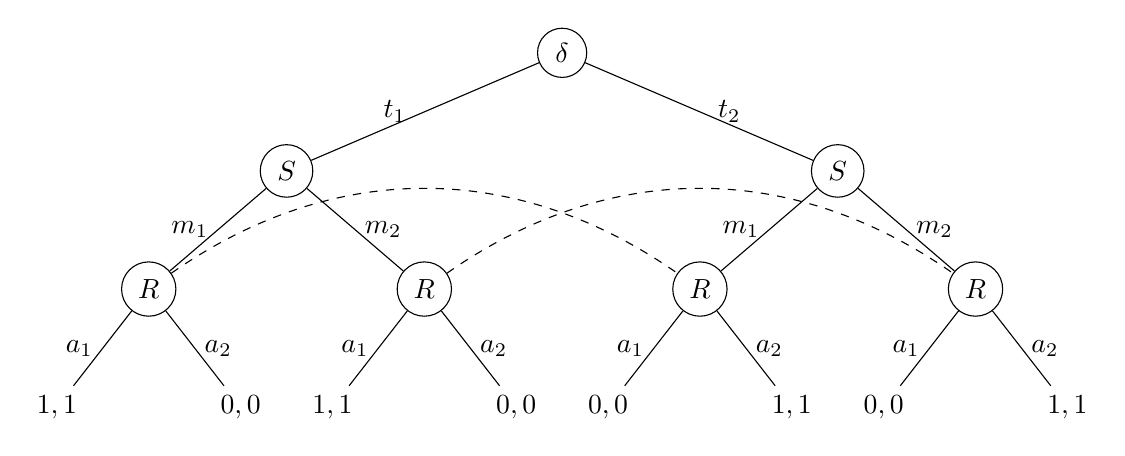
\begin{tikzpicture}[scale=1, level/.style={sibling distance=70mm/#1}]
\node  (z)[circle,draw]{$\delta$}
  child {node [circle,draw] (a_left) {$S$}
    child {node  [circle,draw](left_left) {$R$}
      child {node {$1,1$}        
      edge from parent
		node[left] {$a_1$}
		node[right] {}} 
      child {node (n){$0,0$}
      edge from parent
		node[left] {}
		node[right] {$a_2$}}
    edge from parent
	node[left] {$m_1$}
	node[right] {}}
    child {node  [circle,draw](left_right) {$R$}
      child {node {$1,1$}        
      edge from parent
		node[left] {$a_1$}
		node[right] {}} 
      child {node (n){$0,0$}
      edge from parent
		node[left] {}
		node[right] {$a_2$}}
    edge from parent
	node[left] {}
	node[right] {$m_2$}}
  edge from parent
	node[left] {$t_1$ $ $}
	node[right] {}
  }
 child {node [circle,draw] (a_right) {$S$}
    child {node  [circle,draw](right_left) {$R$}
      child {node {$0,0$}        
      edge from parent
		node[left] {$a_1$}
		node[right] {}} 
      child {node (n){$1,1$}
      edge from parent
		node[left] {}
		node[right] {$a_2$}}
    edge from parent
	node[left] {$m_1$}
	node[right] {}}
    child {node  [circle,draw](right_right) {$R$}
      child {node {$0,0$}        
      edge from parent
		node[left] {$a_1$}
		node[right] {}} 
      child {node (n){$1,1$}
      edge from parent
		node[left] {}
		node[right] {$a_2$}}
    edge from parent
	node[left] {}
	node[right] {$m_2$}}
  edge from parent
	node[left] {}
	node[right] {$ $ $t_2$}
  };

\draw [dashed](left_left) to [out=35,in=-215] (right_left);
\draw [dashed](left_right) to [out=35,in=-215] (right_right);
\end{tikzpicture}
\caption{\textbf{Signaling Game:} Two states, messages, and actions. }
\label{SG1}
\end{figure}
As alluded to above, with the exception of the topmost node and the leaves, all other nodes are \emph{decision nodes}. That is, they represent those points in the game where a particular player must make a decision. An \emph{information set} consists of a set of decision nodes for a given player, which that player cannot distinguish. For example, the receiver is in an information set after hearing $m_2$. She is not sure whether she is in the node beneath state $t_1$ or $t_2$ and she must choose between $a_2$ and $a_2$. She is likewise uncertain after receiving message $m_2$. Again, her inability to distinguish the two states is indicated by a dashed line. An information set can also consist of a single decision node. For example, the sender is never uncertain about the state he is in. Thus the information sets for the sender only ever consist of a single node. 

For each player, a \emph{strategy} specifies which action to take at all \emph{information sets} for a player.\footnote{For simplicity, we only consider \emph{pure} sender (receiver) strategies, functions from states to messages (messages to actions). \emph{Mixed} strategies are a straightforward generalization. A mixed sender strategy specifies a probability distribution over pure sender strategies, $\sigma = p_1 s_1 + ... + p_k s_k$, where $\sum_i p_i = 1$. Similarly, a mixed receiver strategy specifies a probability distribution over pure receiver strategies, $\rho = q_1 r_1 + ... + q_k r_k$.} We will refer to the set of all such sender strategies as $S : [T \rightarrow M ]$, and the set of all such receiver as $R : [M \rightarrow A]$. The set of possible combinations of sender and receiver strategies constitute \emph{strategy profiles}. That is, a sender strategy in the set of possible sender strategies, $s \in S$, and a receiver strategy in the set of all possible receiver strategies, $r  \in R$, yield 
a strategy profile $\langle s,r \rangle$.

Each strategy profile determines the outcome of the game. Crucially, each player's utility function depends on the state of the sender and the action taken by the receiver. That is, their respective utilities are a function of state and action. As an example, consider the case where both sender and receiver prefer successful communication. Then they both receive their preferred payoffs if there is some correspondence between the sender's state and the receiver's action. For example, in Figure \ref{SG1} both sender and receiver prefer the state and action to be the same in the following sense.

\begin{equation}
 U_{S}(t_i, a_k) = U_{R}(t_i, a_k) =
\left\{
	\begin{array}{ll}
		1  & \mbox{if } i = k \\
		0 & \mbox{else}
	\end{array}
\right.
\end{equation}
Note that this reflects the assumption that both sender and receiver have the same preference over outcomes.

Given that the different states occur with certain probabilities, and we are interested in how particular strategies do on average, we consider the \emph{expected utility} for a given strategy profile. This is simply the expected value of the utility functions given the two strategies, which can be given in the case of a discrete state space as in our example above.

\begin{equation}
\begin{split}
 E[U_{S}(s,r)] &= \sum_{t} \delta (t) \cdot U_S(t, r(s(t)))\\
 E[U_{R}(s,r)] &= \sum_{t} \delta (t) \cdot U_R(t, r(s(t)))
\end{split}
\end{equation}
For each possible state the sender and receiver strategies determine an outcome. $s(t)$ is the message the sender will employ and $r(s(t))$ is the action the receiver will take given that message. The expected utility is the sum of these outcomes weighted by the probability of the state that yields them. With these components in place we can now turn to defining the notion of equilibrium and its role in the framework.


\subsection{Equilibria}

A game by itself does not constitute a model in the technical sense. It is a mathematical structure that describes the players preferences and actions, but it does not predict their behavior \emph{per se}. To do so it must be supplemented with a \emph{solution concept} that predicts the conditions under which particular outcomes will obtain. Perhaps the most widely used solution concept is that of a \emph{Nash equilibrium}, which specifies when players have an incentive to unilaterally deviate from a given strategy profile.

\begin{definition}
 A strategy profile $\langle s^*, r^*\rangle$ is a \emph{Nash equilibrium}
if and only if:
  \begin{itemize}
   \item For all $s \in S$, such that $s \neq s^*$, $E[U_S(s^*,r^*)] \geq
E[U_S(s,r^*)]$
  \item For all $r \in R$, such that $r \neq r^*$, $E[U_R(s^*,r^*)] \geq
E[U_S(s^*,r)]$
  \end{itemize}
\end{definition}

The two conditions simply state that neither the sender nor the receiver can do better by individually changing his or her strategy from the equilibrium profile.  The sender's strategy is his \emph{best response} to the receiver's strategy, and the receiver's strategy is likewise her best response to the sender's strategy. Note that these best responses need not be unique to consitute an equilibrium. This follows from the fact that the inequalities in the definiton are not strict. We can, however, impose uniqueness in these best responses by requiring that the inequalities in the definition be strict. A \emph{strict Nash equilibrium} results, meaning that players can only ever do worse if they unilaterally deviate from the equilibrium. Strict Nash equilibria are thus a proper subset of Nash equilibria.

Since we are interested not just in the behavior of a given sender and receiver, but rather the aggregate behavior of a population, we want a broader notion of equilibrium. In particular, we might ask whether a given population is susceptible to change. When considering \emph{asymmetric games}, such as signaling games, where players have different roles, we are actually concerned with two populations: a sender population and a receiver population. To determine the stability of the two populations we can consider a \emph{symmetrized} version of the signaling game, where individuals act as both sender and receiver. A strategy in the symmetrized game is thus a strategy profile of the asymmetric game.

For a population playing the symmetrized game, change depends on whether a given strategy is an \emph{evolutionarily stable strategy} \citep{maynard-smith-price:1973}. Loosely speaking, a strategy is evolutionarily stable if it is resistant to invasion by alternate strategies. That is, when an entire population plays the incumbent strategy the incumbents do at least as well as a mutant. If the mutant does as well, then the incumbent strategy should do better than a mutant in an all-mutant population.  In this case a mutation can be interpreted either in the biological sense or in terms of cultural innovation, such as the introduction of new linguistic signal. The relevant criterion for stability is actually quite simple. For symmetrized asymmetric games, a strategy profile is  evolutionarily stable if and only if it constitutes a strict Nash equilibrium in the original asymmetric game \citep{selten:1980}. That is, mutant senders and receivers only ever do worse than the incumbent strategies. 

For the Lewisian signaling game described above, where states are equiprobable, $\delta(t_1) = \delta(t_2) = \frac{1}{2}$, the only strict equilibria are those where senders employ different signals for each state, and receivers map those messages to the appropriate actions. In other words, the senders \emph{separate} themselves and receivers respond accordingly. These equilibria are referred to as \emph{separating equilibria}. There are also equilibria where senders \emph{pool} themselves together and use only a single message. Receivers are indifferent between actions; they receive the same expected utility for taking either action. These are referred to as \emph{pooling equilibria}. Note that these pooling equilibria are not strict insofar as any action taken by the receiver yields the same expected utility. Thus, in the case of perfectly-aligned interests, separating equilibria are the only evolutionarily stable strategies.


\subsection{Dynamics}

While the term suggests a dynamic interpretation, equilibria, including evolutionarily stable strategies are essentially a static solution concept. They tell us whether a strategy is resistant to invasion or innovation, but tell us nothing about where the populations go to from there. To understand how a population changes over time, a particular \emph{game dynamics} must be supplied. These provide a  description for how a population, or populations, changes from one point in time to the next. Here we use the replicator equations as our game dynamic.

Originally developed as a model of biological replication under selection \citep{taylor-jonker:1978}, the replicator equations are appealing for a number of reasons. First, they are the most extensively studied dynamics and share a number of mathematical properties with a larger set of game dynamics \citep{hofbauer-sigmund:1998}.  This makes establishing results and connecting them to a broader class of dynamics more straightforward. Second, they have a natural interpretation as a form of learning or cultural imitation \citep{fudenberg-levine:1998} and have found broad application in modeling economic \citep{samuelson:1997, cressman:2003} and social behavior \citep{skyrms:1996,skyrms:2004,skyrms:2010}.

The intuition behind the replicator equations is that  more successful strategies increase in frequency. In particular, strategies that are more successful than the population average increase in share of the population. For example, let $\mathbf{x}$ and $\mathbf{y}$ represent the composition of a sender and receiver population respectively. $x_i$ represents the proportion of senders who use strategy $s_i$, and $y_i$ represents the proportion of receivers who use strategy $r_i$. The change of $x_i$ in the population, $\dot{x}_i$, can be given as the following where $f_i(\mathbf{y})$ is the expected utility of $s_i$ given the receiver population, and the average sender expected utility is given as $f(\mathbf{y}) = \sum_{i} x_if_i(\mathbf{y})$.

\begin{equation}
     \dot{x}_i = x_i(f_i(\mathbf{y}) - f(\mathbf{y}))
\end{equation}
The parallel formulation for receiver strategies is then the following, $g_i(\mathbf{x})$ is the expected utility of $r_i$ and $g(\mathbf{x}) = \sum_{i} y_ig_i(\mathbf{x})$.

\begin{equation}
     \dot{y}_i = y_i(g_i(\mathbf{x}) - g(\mathbf{x}))
\end{equation}

Sender and receiver strategies that do better than average have a positive derivative and thus increase. Sender and receiver strategies that do worse than average have a negative derivative and thus decrease. The \emph{rest points} of the dynamics are compositions of the respective populations that do not change from one point in time to the next. Note that by definition Nash equilibria constitute rest points of the dynamics. Neither senders nor receivers have an incentive to deviate from their respective equilibrium strategies. Thus, the average expected utility is identical to the expected utilities of the equilibrium strategies, and the composition of the population does not change.

While we noted that the pooling equilibria in the game described above are not evolutionarily stable strategies, the game dynamics yield further information. That is, the pooling equilibria are saddle points of the dynamics. Almost any small deviation from them leads the population to converge to one of the separating equilibria, which are evolutionarily stable strategies. Crucially, any small difference in the response of receivers to the different signals allows for a kind of tie-breaking. Senders respond to the receivers differentiation by separating, and the population as a whole moves towards one of the separating equilibria.

% The structure of the signaling game along with the game dynamics specify the trajectory of the population over time through a large dimensional space. By definition, evolutionarily stable strategies constitute rest points of the replicator equations. But, in those cases where no evolutionarily stable strategies exist, the game dynamics specify the long-term behavior of the population by allowing us to characterize the stability properties of existing rest points.


\section{Cycles}
\label{Cycles}

We are now in a position to bring the formal framework developed in Section \ref{Signaling} to bear on the use of emphatic negation and its role in Jespersen's Cycle. We begin by first mapping the components discussed in Section \ref{Background} onto the structure of a signaling game. The possibility of different preferences for speakers and hearers is incorporated into the structure of the model. We determine the existence of evolutionarily stable strategies and note the transfer of information as the interests of speaker and hearer diverge. As the preferences of speakers and hearers diverge signaling becomes less informative. For sufficiently low differences, signaling remains informative, but beyond a certain point signaling collapses into uninformative pooling. We then consider the impact of introducing new signals, which lead to a kind of push-chain where the least informative signal is lost. Throughout, we discuss the implications of the model for Jespersen's Cycle.

\subsection{Signaling Game}

To begin, we must first consider how signaling games capture the use of negation. As we noted above, the difference between plain and emphatic negation is captured by the standard of precision applied. The speaker has knowledge about some state of the world which renders a particular negative expression acceptable on some standards, but not necessarily on others. Thus, there exists a continuum of states for the speaker, which we will take to be the interval $T = [0,1]$. The lowest possible value on such an interval corresponds to the weakest possible standard of precision that would still render the negative expression acceptable.\footnote{Here we leave out the possibility of the use of a given expression in the absence of any standard of precision being met. That is, we leave out cases of outright lying. Such cases are particularly interesting, but we leave them as a consideration for future study.} The highest possible value on the interval is then the strictest possible standard of 
interpretation available. 

Given that the speaker has observed some state of affairs, $t \in T$, he must choose a message, $m \in M$, to send to the hearer. Let $\mathcal{P}_n(T)= 0 < ... < t_{n-1} < ... < 1$ be a partition of the state space into $n$ subintervals.  A speaker's strategy is then a function from a partition of the type space to messages, $S : [\mathcal{P}_n(T) \rightarrow M]$. Intuitively, this is simply a way of carving up the state space into discrete regions and using those regions to determine which signal to send. For example, the trivial partition, $\mathcal{P}_1(T)$, occurs when the sender pools all types together and uses only a single message. In what follows we will largely be concerned with partitions of at least size two $\mathcal{P}_2(T)$. For example, consider the case of two messages, consisting of just a plain and an emphatic form. Letting $\mathcal{P}_2(T) = 0 < t_1 < 1$, a possible sender strategy is then  $s(t) = m_1$ for $t \in (0,t_1)$, and $s(t) = m_2$ for $t \in (t_1,1)$. That is, the sender uses 
$m_1$ for all types in the first subinterval, and $m_2$ for the second subinterval. Intuitively, we would refer to $m_1$ as the plain form of negation and $m_2$ as the emphatic.

Once the speaker has sent a message, the hearer is faced with the problem of how to interpret it. Given that the hearer cannot read the speaker's mind, she must infer the state of affairs that prompted the use of a particular form. That is, given the information conveyed by the signal, she must do her best to determine the standard of precision that warrants the speakers assertion. We will take the space of possible interpretations available to the hearer to be equivalent to the type space of the speaker, $A = [0,1]$. This representation captures the fact that the interpretation of expressions is not an all or nothing affair, but rather a matter of degrees.  A hearer's strategy is then a mapping from messages to interpretations, as above, $R : [M \rightarrow A]$.

With the definition of the strategies available to speakers and hearers, we can ask what kinds of preferences both might have over the correspondence between actual and inferred standards. It is uncontroversial that hearers are in the business of doing their best to accurately infer the actual state of affairs that prompted the signal. That is, hearers prefer their interpretation to be as close as possible to the standard of precision that the speaker actually has evidence for.  If it were otherwise, the existence of language would be truly puzzling from an evolutionary perspective; the gullible are not long for the tooth and claw world. So, if hearers are interested in the accurate transmission of information, then any misalignment must come from speakers' preferences. 

From the perspective of the speaker, we can adduce at least two related reasons why speakers might prefer overestimation. The first imputes a kind of categorical bias on the part of speakers, whereas the second relaxes this bias towards reasonability. We address them each in turn. First, we consider what the goals of communication are. Arguably, our chief goal in uttering a given expression is to affect some response in our interlocutors. In the case of a declaration we might think of this in terms of how convinced the hearer is after hearing an utterance. Or, in the terms we have developed thus far, we want the hearer to infer a particular standard of precision. We could take this preference as categorical. Namely, that regardless of the actual standard of precision, speakers want hearers to infer the absolute highest standard of precision possible. Given such a preference and a choice between signals that hearers respond to differentially, speakers will always choose the form that elicits the higher 
standard.  Speakers are, so to speak, on the lookout for the form that gives them the most bang for their breath. It should be noted that this bias is stipulative only insofar as it arises from the fundamental way we use words to do things.

Second, while this bias may naturally exist, it need not be categorical. Rather, speakers may simply prefer that hearers infer a standard of precision that is at least is strict as their own. This can be taken as a natural corollary of the inferential nature of communication. Hearers cannot read minds, and thus they must make some inference about the actual standard of precision. Speakers have only an indirect influence on this process of inference. Thus, they may wish to hedge their bets in a particular direction. Namely, they may want the inferred standard to be at least as strict as there own because it ensures that their own beliefs stand in a particular relation to hearers'. That is, the hearer's beliefs probabilistically entail those of the speaker.

The impact of this relationship is particularly clear with regard to perlocutionary concerns. For example, imagine the case where the issuer of one of the following threats has absolutely no desire to follow through on it.

  \ex. \a. If you move, I'll shoot.
       \b. If you budge an inch, I'll shoot.

By using the stronger threat, leading the hearer to infer a stricter standard than actually holds, the speaker has a better chance of not being forced to follow through on it. That is, the hearer will restrict his actions to those that do not constitute movement at the stricter standard, thus guaranteeing that they will not at the weaker actual standard. 

The same concerns hold in far more magnanimous circumstances. For example, in the case of offering a friend genuine advice on dining options, one might deem a mediocre restaurant one of the following.

 \ex. \a. Not good.
      \b. Not worth a cent!

While clearly hyperbole, the latter, much like the strong threat, offers a means for speakers to guide a friend to a good meal. In both cases, when hearers underestimate the standard of precision, the speaker runs the risk of not achieving his goals with resulting dire or not so delicious consequences. In contrast, these goals are guaranteed when hearers overestimate the standard of precision.

We can encode this slight bias in the utility functions of senders and receivers. As a means of parameterizing this possibility, we define the sender and receiver utility functions as a pair of quadratic functions, as in \cite{crawford-sobel:1982}, where $b \in [0,1]$ reflects the bias of the sender.\footnote{This bias need not be constant. For example, we might suppose that the bias is uniformly distributed over the interval $(t,t+b)$. This would capture the intuition that some of the time a speaker prefers overestimation of the standard, but not others. All of the following result hold for this more general case. As a preview, the only change below is that partial pooling equilibrium is defined at $t^* = \frac{1}{2} - 3b$ }

\begin{equation}
\begin{split}
     U_S(t, a) &= -(a - t - b)^2\\
  	 U_R(t, a) &= -(a - t)^2
\end{split}
\end{equation}
These utility functions reflect two intuitions. First, for a given type of sender, there is an action that maximizes the receiver's payoff. That is, the receiver does best by taking the action that is closest to the sender's type. Second, for a sender with a particular type, the action that maximizes the sender's payoff is offset by some bias, $b$. That is, the sender prefers the receiver to take the action she thinks appropriate for some higher type. In this case, $b$ represents the degree to which the sender wishes to exaggerate his type, if the receiver believes such exaggerations. When $b=0$ the interests of senders and receivers are completely aligned, but as $b$ grows, they diverge. This parallels the intuition that hearers are trying to infer the standard of precision for a given assertion, and prefer this to be as accurate as possible. It also reflects the fact that speakers have a slight preference for hearers to overestimate the standard of precision.

The impact of the sender's bias can be visualized as in Figure \ref{receiver_payoff}. For a sender with information $t=0$, the receiver would do best to take the action that accurately picks out the sender's state. In contrast, the sender's most preferred action is offset by the amount of bias. In the case where $b=\frac{1}{2}$, then the sender prefers the speaker to take an action higher than the receiver would prefer. This mismatch is only exacerbated as the amount of bias increases, as can be seen for the case where $b=1$. Visually speaking, as the bias increases, the utility functions of the sender and the receiver move away from each other. 

\begin{figure}
\begin{center}
     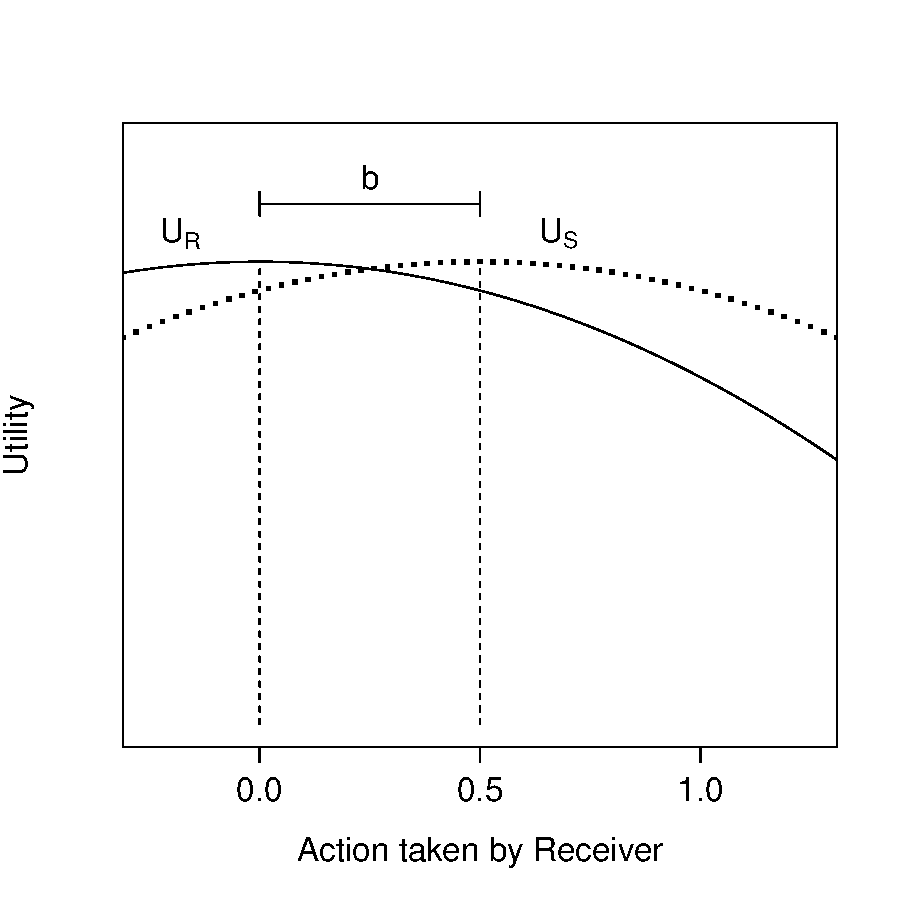
\includegraphics[width=3in]{payoffgraph2.pdf} \hspace{.5cm} 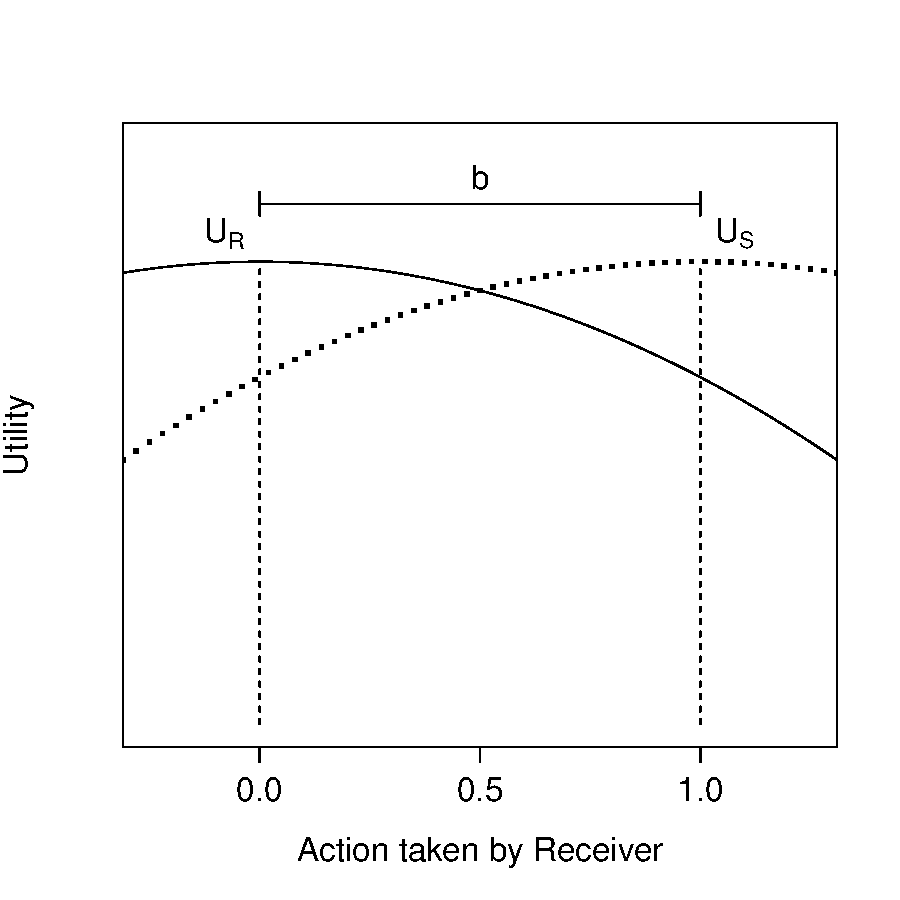
\includegraphics[width=3in]{payoffgraph.pdf}
\end{center}
\caption{Sender and receiver utility functions for $t=0$ and $b=\frac{1}{2}$ (left) and $b=1$ (right)}
\label{receiver_payoff}
\end{figure}

\subsection{Equilibria}

For a given pair of sender and receiver strategies we can calculate the expected utility. In what follows we will assume that types are uniformly distributed over the interval, which yields the following expected utilities. Note that these are exactly parallel to expected utilities in a discrete state space presented above.

\begin{equation}
\begin{split}
     E[U_S(s, r)] &= \int_T -(r(s(t)) - t - b)^2 dt\\
      E[U_R(s, r)] &= \int_T -(r(s(t)) - t)^2 dt
\end{split}
\end{equation}

Now, we want to determine the conditions for equilibria. By doing so, we are determining what kinds of behavior we would expect on the part of speakers and hearers given the speaker's bias. That is, we want know how speakers will use different forms to signal standards of precision and how hearers will interpret them. The existence of different equilibria and their relative stability are crucial to the dynamics of Jespersen's Cycle.

Consider the potential equilibrium strategy profile $\langle s^*, r^* \rangle$. Let $s^*$ induce a partition of type $\mathcal{P}_2(T)$, where $t^*$ is the relevant threshold that distinguishes the two messages. Let $s^*(t) = m_1$ for $t \in (0,t^*)$ and $s^*(t) = m_2$ for $t \in (t^*,1)$. Let $r^*(m_1) = a_1^*$ and $r^*(m_2) = a_2^*$. In words, the sender splits the type space in two and sends a unique message for each subinterval. These are the plain and the emphatic forms of negation, respectively. The receiver responds to these messages with a particular action.  These are the inferred standards of precision in response to the different forms.

The strategy profile is an equilibrium if the relevant strategies are joint best responses. We can determine this by simply taking the partial derivative of the relevant utility functions with regard to the relevant variables. For the receiver, this can be determined by considering what actions are the best response to the senders partition. This simply tells us how the receiver's inference depends on the sender's use of the different forms.

\begin{equation}
\frac{\partial}{\partial a_1^*}E[U_R(s, r)] = \frac{\partial}{\partial a_2^*}E[U_R(s, r)] = 0
\end{equation}
These values are uniquely satisfied when the following hold.

\begin{equation}
     \begin{split}
	  a_1^* &= \frac{t^*}{2}\\
	  a_2^* &= \frac{1 + t^*}{2}
     \end{split}
\end{equation}
Intuitively, this means that however the speaker splits up the standards of precision, the receiver should respond to the emphatic form by inferring a higher standard of precision and the plain form with a lower standard of precision. The exact placement of these responses is determined by how the sender uses the signals. Namely, the hearer should infer the average standard of precision used for each of the two forms.

For the sender, we can proceed in a similar fashion determining when the following holds.
\begin{equation}
 \frac{\partial}{\partial t^*}E[U_S(s, r)] = 0
\end{equation}
This equation is satisfied when one of the following holds.

\begin{equation}
     \begin{split}
 	t^* &= 0\\
	t^* &= \frac{1}{2}(a_1^* + a_2^*) - b\\
	t^* &= 1
     \end{split}
\end{equation}

These constraints together give rise to three distinct systems of equation. Solving each for $t^*$, we find the following equilibrium solutions in terms of the bias of the sender.

\begin{equation}
\begin{split}
     t^* &= 0\\
     t^* &= \frac{1}{2} - 2b\\
     t^* &= 1
\end{split}
\end{equation}
Both the first and the last of these equilibria are pooling equilibria. That is, senders only ever use a single signal. In response to this, receivers take the action that maximizes their expected utility given the prior probability distribution over types. That is, they guess the expected value of the type space. They simply infer the average standard of precision.

In contrast, the middle equilibrium constitutes a partially separating equilibrium. It is only partially separating because the state space is infinite, while the message space is not. This means that every type cannot be fully revealed, but that some information is transferred. The amount of information transferred and the distinction between the partially separating and pooling equilibria can be characterized in information-theoretic terms \citep{shannon:1948}. In particular, we can think of the amount of information conveyed by a particular signal at equilibrium according to the \emph{Kullback-Leibler Divergence} \citeyearpar{kullback-leibler1951divergence}.

\begin{equation}
     D_{KL}(P || Q) = \int_{-\infty}^{\infty} log\left( \frac{p(x)}{q(x)}  \right)p(x) dx
\end{equation}
This serves as a measure for how much change is induced in the receiver by a particular message. That is, in our case $q(x)$ corresponds to the prior probability distribution over types, and $p(x)$ corresponds to the probability of a sender being of a particular type given the message. The more the message shifts the probability from the prior, the more information it conveys. And, the less a message shifts the probability from the prior, the less information it conveys. 

For example, taking either of the pooling equilibria as an example.  If senders use the same signal regardless of state, then the conditional probability is the same as the prior probability. This means that there is absolutely no change from the prior probability, and hence zero information is transmitted via the signal. In contrast, for any partially separating equilibrium, a particular message induces a shift from the prior probability, and thus conveys some information. We should note that the amount of information conveyed regarding the standard of precision is distinct from the propositional content of a given utterance. For example, in the case where speakers use only a single form of negation for all standards of precision, the hearer will have no information in addition to and exceeding the prior probability. However, she will know the propositional content of the utterance. In other words, she will know \emph{that} negation was used, but not \emph{how} it was used.


Information is transferred at equilibrium only if the partially separating equilibrium exists. This is the case when the sender's bias is sufficiently low. Namely, only if $b < \frac{1}{4}$. If the bias is too large, then the partially separating equilibrium collapses into the lower pooling equilibrium.  However, a partially separating equilibrium, if it exists, is the only evolutionarily stable strategy profile. To see this note that in any pooling equilibrium receivers can respond to an unused message with any action whatsoever without affecting their expected utility. This means that pooling equilibria are not strict Nash equilibria and are thus not stable to invasion or innovation. 

% For example, suppose that receivers responded to an unused message with an action $a > \frac{1}{2}$. All senders would then do better to use that previously unused message in a particular set of states, $(\frac{1}{2}(a + \frac{1}{2}), 1]$. In turn, receivers woul
% 
%  have an incentive to adjust their responses to the two messages. In turn, senders have an incentive to adjust to this adjustment, and so forth. This process of mutual adjustment ends at the evolutionarily stable partially separating equilibrium.

We have established an upper limit on the amount of bias that allows for two signals to be used informatively. If this bias is exceeded, then signaling collapses. A single message is used, but carries no information. In fact, for a given number of signals, $n$, there exists some level of bias, $b_n$, that allows for their informative use in a partially separating equilibrium based on a sender's partition of the type space, $\mathcal{P}_n$ \citep{crawford-sobel:1982}. As the number of signals increase, the amount of bias must decrease to allow for informativity, thus $b_2 > b_3 > ... > b_n$. Intuitively, as the preferences of senders and receivers approach each other a finer and finer partition of the space is possible.

\subsection{Dynamics}

So, what does this mean for Jespersen's cycle? Intuitively, the pragmatics of emphasis suggest that the population originally starts at a point where one form is used with a  very high standard of precision and another is used for all other standards. That is, emphatic negation is distinguished from plain negation in its contexts of use. We can determine what will happen to these two signals over time. Intuitively, under the game dynamics, the signals will converge to their equilibrium use.

Under the game dynamics, for any amount of bias, no matter how slight, the emphatic form will spread to lower and lower standards of precision until it reaches its equilibrium use. The amount of bias determines where this process stops. That is, if a partially separating equilibrium exists, then the emphatic form will expand to encompass all standards of the upper part of the partition. In other words, the emphatic will be \emph{attenuated}, but still carry some information.  If no separation is possible, the emphatic form will spread across all standards. In other words, the emphatic will be entirely \emph{bleached} of its emphasis. Note that in both cases the process can be characterized in information-theoretic terms. That is, as the emphatic form spreads to more and more standard it conveys less and less information. 

The stable coexistence of plain and emphatic negation for long periods of time suggest that the bias is sufficiently small to allow for at least two forms. This, however, raises the question of what destabilizes the system. The system must be disturbed by a push chain, whereby the signal used for the lowest subinterval is lost. More generally, imagine a system with bias $b_n$ at equilibrium. Now, suppose that a new signal is introduced, so that there are now $n+1$ signals. Clearly, the system is not stable. However, it will be carried back to some equilibrium by the game dynamics. The resultant equilibrium depends on the character of the signal that is introduced. Let $a'$ be the response of receivers to the new signal $m'$. All messages that receive a lower response than $a'$ will be pushed down, the lowest of these being pushed out of use completely.  In the case of Jespersen's Cycle, new signals enter with a high $a'$, and thus displace everything below. That is, they are emphatic and lead hearers to 
infer a high standard of precision. This means that all other forms lower in the scale will be pushed down and the lowest will be pushed out of existence, exactly like what we see in the actual instantiation of the cycle.

\subsection{Future Directions}

This analysis suggests how Jespersen's Cycle can arise from signaling under a slight speaker bias. Examining the effect of these pragmatic pressures we established the following results. First, we showed that, for any amount of bias, emphatic forms become less informative over time. The extent of this loss is governed by the amount of bias, ranging from attenuation to complete bleaching. Second, only finitely many signals are stable in equilibrium for a given amount of bias.  The introduction of additional signals results in a push-chain scenario whereby the least informative signal is lost and the population returns to equilibrium. 

There are several further directions that remain to be explored. First, we have encoded a bias on the part of the speaker into the utility function. This gives rise to the inflationary effect whereby emphatic negation is attenuated. However, it is not clear that this effect need arise from the speaker's preferences. For example, it may be the case that it could equally as well arise from the speaker's uncertainty regarding the hearers beliefs about the distribution over standards of precision. Thus far, we have relied on the \emph{common prior assumption}, which allows for the reduction of games of incomplete information to games of imperfect information \citep{harsanyi:1967,harsanyi:1968a,harsanyi:1968b}. That is, we have assumed that both speaker and hearer share the same prior probability over standards of precision. This need not be the case, but it is an open question as to whether removing this restriction yields a qualitatively different result than the course pursued here. Further, given every 
individual's experience as both a sender and a hearer, the common prior assumption may be well justified.

Second, we have assumed a uniform prior distribution over the state space. This serves well enough as a starting point, but the interaction between distributions and biases may yield dramatically different constraints than those discussed above. A straightforward generalization could be had by considering the \emph{Beta Distribution} over the state space, of which the uniform distribution is a special case. This would allow for a wide ranging test of the interaction between the prior probability and the amount of information that can be conveyed. Finally, the generalization of the prior can be informed in part by an empirical investigation of how often emphatic negation actually occurs. For example, if, as we have suggested, emphatic negation arises from NPIs in focus then we should be able to estimate the overall rate of use by determining how often such NPIs bear the mark of an abstract focus feature. That is, we can compare the overall rate of negation to the occurrence of NPIs with prosodic prominence.  
While this only indirectly tells us about the underlying distribution of standards of precision, it provides a kind of constraint that will allow us to estimate likely distributions.


% \begin{itemize}
%  \item Common prior assumption
%  \item Uncertainty over receiver type
%  \item Shape of prior
% \end{itemize}


% The introduction of signals at different points in a scale parallels the distinction between Jespersen's Cycle and the \emph{Quantifier Cycle} \citep{haspelmath1997}. That is, 

%  The result of introducing the new signal is a partially separating equilibrium where the signal with the lowest standard of interpretation is lost, but everything else is as before. To borrow a metaphor from sound change, the least informative signal is replaced by a \emph{push chain}. If new signals are coming in from above, then we would expect a 
% consistent transition down the standards of interpretation. However, this does not preclude the introduction of signals at other points on the scale. We would simply predict a different outcome.


% scale-reversing

\section{Stability}
\label{Stability}


The analysis presented in the previous section suggests that pragmatic pressures can lead to the increase in the use of a postverbal negator. The question is then why this increase so often leads to the loss of the preverbal negator. If, at some point, the postverbal negator comes to be negative in its own right, then this clearly impinges on the process of acquisition. Learners are faced with the problem of determining what exactly expresses negation. Here we examine how use and acquisition might allow for the transition from preverbal negation to postverbal negation. We consider whether the two mechanisms can independently bring about the change, or whether they must act in concert to destabilize the current system of negation.

At the heart of this question is the amount of evidence that a given element expresses negation. At the beginning of the change clearly only the preverbal negator does so. The postverbal reinforcer only emphasizes this negation. Eventually though, the evidence weighs in favor of the postverbal negator alone being the expression of negation. \cite{wallage2008} characterizes this transition in morphosyntactic terms as the loss of a [+NEG] feature on the preverbal negator, along with the concomitant introduction of a [+NEG] feature on the postverbal negator. This then allows for the loss of the preverbal negator given that the negative feature can be found elsewhere in the sentence.

We can formulate the effect of various amounts of evidence in terms of Yang's \citeyearpar{yang:2002} variational model. First, let there be two grammars, $G_{ne}$ and $G_{not}$, that represent the location of the abstract feature at \emph{ne} and \emph{not} respectively. We can represent the relation between the two grammars schematically as in Figure \ref{grammars}. In this case, $\alpha$ indicates the proportion of the linguistic environment that is only compatible with $G_{ne}$, and $\beta$ indicates the portion of the linguistic environment that is only compatible with $G_{not}$. The proportion of the two grammars in the population is governed by the following learning rule, where $p_0$ and $p_t$ represent the proportion of $G_{ne}$ in the population after $0$ and $t$ generations, and $q_0$ and $q_t$ represent the proportion of $G_{not}$ after $0$ and $t$ generations.

\begin{equation}
     \frac{q_t}{p_t} = \left( \frac{\beta}{\alpha} \right)^t\frac{q_0}{p_0}
\end{equation}

\begin{figure}
\begin{center}
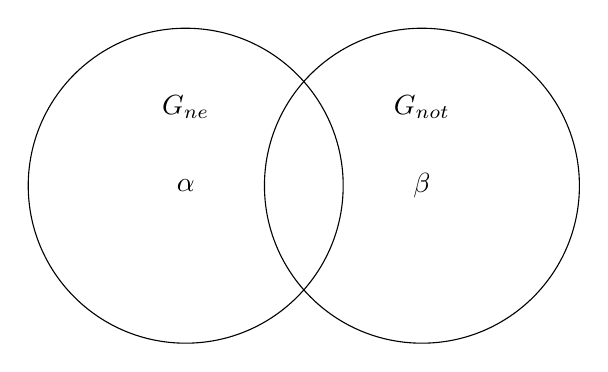
\begin{tikzpicture}
  \tikzset{venn circle/.style={draw,circle,minimum width=#1}}
  
  \node (A) [venn circle = 4cm]  at (0,0) {$\alpha$};
  \node (G1) [above of=A] {$G_{ne}$};
  \node [venn circle = 4cm] (B) at (0:3cm) {$\beta$};
  \node (G2) [above of=B] {$G_{not}$};
%   \node[below] at (barycentric cs:A=1/2,C=1/2 ) {$G_1 G_2$};   
\end{tikzpicture}       
\end{center}
\caption{Two mutually incompatible grammars}
\label{grammars}
\end{figure}


On the standard version of the model, if $\beta \neq \alpha$, then one grammar or the other will win out. Thus, we would expect that starting from a given point in time an incoming grammar would only spread if it had more initial evidence in favor of it. However, this rests on the assumption that no mechanisms other than acquisition are acting on the distribution of forms. Our analysis thus far suggests that this need not be the case.

Here we consider the two mechanisms that might factor into the trajectory of the change. First, the increase of postverbal negation directly impacts the change insofar as it diminishes $\alpha$. Second, there are instances of $ne$ that provide evidence that it does not bear the negative feature, rendering $\beta$ nonzero.  Both mechanisms alone, or in combination can be used to make predictions about the trajectory of the change over time. We consider each mechanism in isolation and then in tandem, determining whether either is sufficient   to cause the change in isolation.

As noted in the previous section, the use of the postverbal negator spreads up to a point, which is determined by the bias of the speaker. At the most, this can result in the reduction of $\alpha$ to $0$. That is, if $ne...not$ is the only form of negation ever used, then there is equal evidence that $ne$ and $not$ express negation. That is, there is no reason why we would expect one form to replace the other. This means that pragmatic pressures are not sufficient in isolation to affect the change. Rather, there must be some precursors that pave the way for the change. This is an interesting, but arguably welcome limitation to the scope of pragmatic pressures. Use can only do so much.  Similarly, unless the evidence is already in favor of $not$ as the expression of negation there is no chance that the change will go through. That is, neither change is sufficient to bring about the change on its own. However, together, the two offer insight into how the change takes place.

We consider how increased use of the postverbal negator might interact independent evidence that $not$ is the expression of negation. Namely, we consider the appearance of all forms in environments that license the appearance of negative polarity items, which are indicative of the lack of the abstract negative feature. These include the scope of negation, certain positions in comparative constructions, antecedents of conditionals (when not expressing actual negation), the restrictor of universal quantifiers, in the scope of verbs of doubting, in embedded clauses under negation, and direct and indirect questions \citep{ladusaw1979, giannakidou1998}. This simply reflects the intuition that NPIs are associated with some negative feature, but not negative in their own right. Occurrence outside these environments can be taken as evidence for the abstract feature. Thus, for both the preverbal and postverbal negators, the amount of evidence that they bear the abstract feature can easily be found for at least some 
of these categories from a corpus. \cite{wallage2008} gives occurrences of the various forms of negation from the Penn-Helsinki Parsed Corpus of Middle English (PPCME2) \citep{ppcme2}  in main clauses, subordinate clauses, \emph{if}-clauses, and in the scope of negation.

\begin{table}[ht]
\begin{center}
\begin{tabular}{@{}cccccccc@{}}
\hline
Main Clauses & & & &Subordinate Clauses &  &   &\\
\hline
Period & \emph{ne} & \emph{ne...not} & \emph{not} & Period & \emph{ne} & \emph{ne...not} & \emph{not}\\
\hline
1150-1250 & 91 & 152 & 3  & 1150-1250 & 279 & 112 & 4  \\
1250-1350 & 48 & 329 & 48  & 1250-1350 & 87 & 147 & 15  \\
1350-1420 & 3 & 108 & 935  & 1350-1420 & 17 & 115 & 905  \\
1420-1500 & 1 & 12 & 928  & 1420-1500 & 7 & 4 & 821  \\
\hline
\end{tabular}
  \caption{Frequency of forms in main and subordinate clauses from}
\end{center}
\end{table}

\begin{table}[ht]
\begin{center}
\begin{tabular}{@{}cccccccc@{}}
\hline
\emph{if}-clauses & & & &In scope of negation &   &   &\\
\hline
Period & \emph{ne} & \emph{ne...not} & \emph{not} & Period & \emph{ne} & \emph{ne...not} & \emph{not}\\
\hline
1150-1250 & 33 & 10 & 0  & 1150-1250 & 33 & 3 & 0  \\
1250-1350 & 12 & 8 & 3  & 1250-1350 & 19 & 6 & 2  \\
1350-1420 & 9 & 5 & 64  & 1350-1420 & 14 & 8 & 55  \\
1420-1500 & 2 & 1 & 51  & 1420-1500 & 4 & 1 & 43  \\
\hline
\end{tabular}
  \caption{Frequency of forms in \emph{if}-clauses and In scope of negation}
\end{center}
\end{table}

Taken together, we can estimate the amount of evidence over time for and against the two grammars. That is, those occurrences of a particular form by itself in a main or a subordinate clause constitute positive evidence for its respective grammar, whereas those occurrences of a particular form in the scope of negation constitute positive evidence for the other grammar. It is not clear whether all the instances of negation in the antecedent of conditionals express negation, so here we leave them out of our counts. The change in the relative evidence across time can be seen in Table \ref{evidence}. 

\begin{table}[ht]
\begin{center}
\begin{tabular}{@{}cccccc@{}}
\hline
Period & $\alpha$ & $\beta$ & $\frac{\beta}{\alpha}$ & \emph{ne...not}\\
\hline
1150-1250 & 370 & 40  & .108 & 277\\
1250-1350 & 137 & 65 & .474 & 490\\
1350-1420 & 75 & 1799 & 23.986 & 236\\
1420-1500 & 51 & 1704 & 33.411 & 18\\
\hline
\end{tabular}
  \caption{Relative evidence for grammars}
\label{evidence}
\end{center}
\end{table}

At some point during the transition from the second to the third period there is a clear tipping point in the amount of evidence for the two grammars. $ne$ goes from being favored as the host of the negative feature to being grossly disfavored. Note that this transition coincides with the peak usage of \emph{ne...not}, suggesting that the increasing use of postverbal negation continued up until a certain point, rendering $not$ the uncontested expression of negation. Both use and acquisition play there parts in bringing about the change.

Now, while this evidence is suggestive, it still leaves the appearance of $not$ by itself a mystery. This follows from the fact that the variational model is not a model of actuation itself. To see this note that the grammar must already be in existence for it to grow. That is, if $q_0 = 0$ then $q_1=0$.

\begin{equation}
     \frac{q_1}{p_1} = \left( \frac{\beta}{\alpha} \right)\frac{q_0}{p_0}
\end{equation}
One possible way of making sense of this actuation stems from the phonetic weight of the preverbal negator. That is, as the postverbal negator increases in frequency, even a small probability of misperceiving the preverbal negator as absent provides evidence for the change, and, importantly, the ultimate loss of the preverbal negator. It might be possible to infer the impact of these misperceptions over time given the predicted dynamics of the learning model. That is, the proportion of a given grammar must exceed a threshold to keep from being effectively washed out by one generation. We can test how a small error rate in misperceptions might counteract this force, and, along with the steady increase in postverbal negation, bring about the eventual loss of the preverbal negator. 

\subsection{Future Directions}

The evidence presented suggests how the cycle depends on both use and acquisition. However, it is far from a complete picture. First, an extensive analysis of the various forms of negation in the PPCME2 will be necessary, both for a more accurate estimate of the evidence for both respective grammars, as well as an overview of the details concerning the various forms of negative elements, including other NPIs, negative adverbs, and negative quantifiers. Second, the relevant grammatical description of the change presented here is quite simplified relative to the more articulated approach discussed in \cite{wallage2008}. Namely, he divides the change in negation into finer parts. $ne$ goes from having interpretable [$i$neg] to an uninterpretable [$u$neg] negative feature. Such an analysis could be incorporated into the learning model presented here and might possibly shed light on the loss of $ne$ and other subsequent changes such as the loss of negative concord. Finally, the analysis of the cycle in Middle 
English could benefit greatly from a comparative perspective. The cycle in French differs widely in terms of both the relevant timeline and the evidence available at the onset of the change. Data from the MCVF Corpus of Middle French \citep{mcvf} could offer an important counterpoint and testing ground for the models presented thus far.

\section{Implications \& Further Considerations}

Pragmatic competence shapes the input to language acquisition, language acquisition gives rise to grammatical competence, and grammatical competence determines the set of signals at the disposal of our pragmatic competence. The goal of this dissertation is to advance our understanding of the relationship between the two as repeated in Figure \ref{second}. By loosening the assumption of perfectly common interests between speakers and hearers, we can gain insight into how the use of linguistic signals changes over time, and how this impacts acquisition. By generalizing the Gricean program we have been able to situate Jespersen's Cycle at the intersection of both. Neither by itself can account for the trajectory of the cycle, but both taken together are mutually informing and revealing.

\begin{figure}
\begin{center}
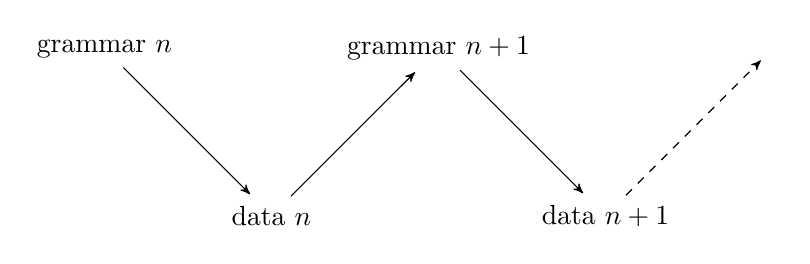
\begin{tikzpicture}[->,>=stealth',shorten >=1pt,auto,node distance=3cm]
  \node (A)      {grammar $n$};
  \node (B) [below right of=A]  {data $n$};
  \node (C) [above right of=B] {grammar $n+1$};
  \node (D) [below right of=C] {data $n+1$};
  \node (E) [above right of=D] {};
\path[->] (A)  edge node {} (B)
  (B) edge node {} (C)
  (C) edge node {} (D)
  (D) edge[dashed] node {} (E);
\end{tikzpicture}
\end{center}
\caption{The iterated process of language acquisition and use}
\label{second}
\end{figure}



\subsection*{Timeline}

\begin{description}
	\item[May-June 2014:] \hfill \\ Pursue further directions regarding signaling model \\  Gather and code data from PPCME2 \\ Analyze results for English data
        \item[July-August 2014:] \hfill \\ Write up signaling model results \\ Write up English results \\ Gather and code data from MCVF
	\item[September-October 2013:] \hfill\\
	Analyze results for French data \\ Write up French results
	\item[November-December 2013:] \hfill\\ Summarize implications for language use \\ Summarize implications for language acquisition 
	\item[January-February 2014:] \hfill\\ Write introduction \\ Write conclusion
	\item[March-April 2014:] \hfill\\ Put together defense \\ Defend (mid April)  \\ Revise as per recommendations \\ Submit (early May)
\end{description}

% \begin{figure}
% \begin{center}
% \begin{tikzpicture}
%   \tikzset{venn circle/.style={draw,circle,minimum width=#1}}
%   
%   \node (A) [venn circle = 4cm]  at (0,0) {$\alpha$};
%   \node (G1) [above of=A] {$G_{ne}$};
%   \node [venn circle = 4cm] (B) at (0:3cm) {$\beta$};
%   \node (G2) [above of=B] {$G_{not}$};
% %   \node[below] at (barycentric cs:A=1/2,C=1/2 ) {$G_1 G_2$};   
% \end{tikzpicture}       
% \end{center}
% \caption{Two mutually incompatible grammars}
% \end{figure}


% \begin{equation}
%      C_i = Pr(G_i \nrightarrow s | s \in E)
% \end{equation}
% 
% \begin{equation}
%      \lim_{t \rightarrow \infty}p = \frac{C_2}{C_1 + C_2}
% \end{equation}
% 
% \begin{equation}
%      p' = \frac{\alpha p}{\alpha p + \beta q}
% \end{equation}
% 
% \begin{equation}
%      q' = \frac{\beta q}{\alpha p + \beta q}
% \end{equation}
% 
% \begin{equation}
%      \frac{q'}{p'} = \left( \frac{\beta}{\alpha} \right) \frac{q}{p}
% \end{equation}
% 
% \begin{equation}
%      \frac{q_t}{p_t} = \left( \frac{\beta}{\alpha} \right)^t\frac{q}{p}
% \end{equation}


% \begin{equation}
%      q_t < \epsilon
% \end{equation}


% \begin{equation}
%      q_0 < \frac{\epsilon}{\left(\frac{\beta}{\alpha}\right)^t + \epsilon}
% \end{equation}



%\bibliographystyle{}
\bibliography{ahern.bib}



\end{document}